\pgfplotsset{compat=newest}

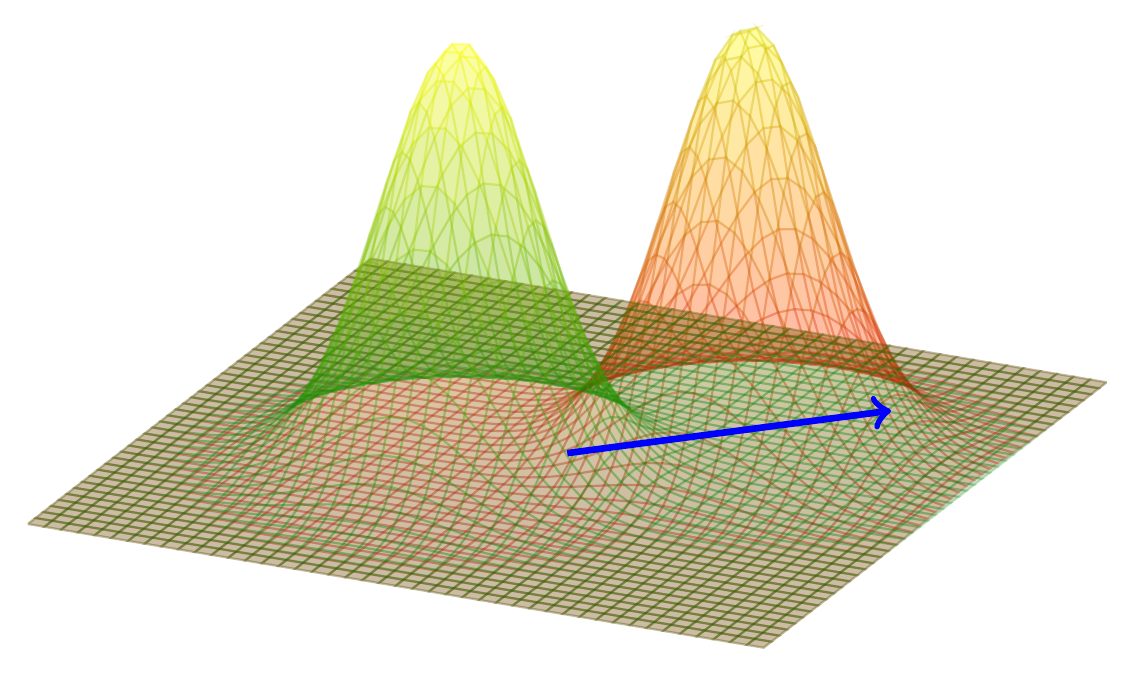
\begin{tikzpicture}[scale=2]
\begin{axis}[domain=-5:5, hide axis]
\addplot3 [surf, opacity=0.2, samples=45, colormap/redyellow] {e^(-((x-2)^2 + (y-1)^2)/2)};
\addplot3 [surf, opacity=0.2, samples=45, shader = flat, colormap/greenyellow] {e^(-((x+1)^2 + (y+1)^2)/2)};

\draw[very thick, blue, ->] (0,0) -- (3,3);

\end{axis}
\end{tikzpicture}
